\chapter{Opis projektnog zadatka}
		
		
		Pronaći lokacije koje su dostojne i prikladne za čovjekovog najboljeg prijatelja nije uvijek lako i jednostavno. Stoga smo u cilju lakšeg pronalaska lokacija pogodnih za ljubimce razvili programsku podršku za web aplikaciju Dog Friendly.
  
		Dog Friendly aplikacija pokazuje svojim korisnicima, vlasnicima i ljubiteljima pasa, korisne lokacije kao što su veterinarske ordinacije i frizerski saloni za pse, ali i lokacije koje nisu prikladne za ljubimce kako bi ih mogli lakše zaobići.
		\newline
		
		Na početnoj stranici korisnik saznaje informacije o ideji web stranice. Odmah ispod tog opisa nalazi se gumb "Karta" koji vodi korisnika na glavnu mogućnost web stranice, a to je prikaz gore navedenih lokacija. Pristup karti imaju registrirani i neregistrirani korisnici. \newline
		
		Svi korisnici (neregistrirani i registrirani) na karti mogu vidjeti lokacije koje su označene kao prikladne ili neprikladne za pse. Kako bi se korisniku olakšalo i ubrzalo traženje informacija pokraj karte su tražilica (za upis adrese i imena lokacije/obrta) i prostor za filtriranje lokacija i obrta po kategoriji.\newline
  
		Na karti se prikazuju markeri kao pokazatelji željenih i neželjenih lokacija. Pritiskom miša na lokaciju označenu markerom korisnik može saznati:
		
		\begin{packed_item}
			\item {ime lokacije}
			\item {ocjenu}
			\item {kategoriju (park, plaža, kafić, restoran, ostalo)}
		\end{packed_item}
		\newline
		
		Registrirane korisnike dijelimo na osnovne korisnike i vlasnike obrta. Prilikom registracije korisniku se objašnjava razlika između navedenih i daje mogućnost odabira.
  
        Obični korisnik, osim funkcionalnosti koje se prikazuju neregistriranim korisnicima, ima mogućnost dodavanja novih lokacija i ocjenjivanja. S druge strane, vlasnik obrta ne može ocjenjivati, ali može promovirati svoj obrt.
		\newline
		
		U slučaju da osoba odabere "Korisnik" (osnovni korisnik) popunjava formu sa sljedećim upitima:
		
		\begin{packed_item}
			\item {korisničko ime}
			\item {e-mail adresa}
			\item {lozinka}
		\end{packed_item}
  
        Pritiskom gumba "Registracija" pristiže joj e-mail koji sadrži link za potvrdu registracije. Klikom na link korisnika se vodi na stranicu za uspješnu registraciju te on time dobiva mogućnost prijave u aplikaciju.\newline 
        
		U slučaju da korisnik prilikom registracije izabere "Vlasnik obrta" za kreiranje računa, uz već navedene podatke korisničkog imena, e-mail adrese i lozinke, potrebni su i sljedeći podaci:
		
		\begin{packed_item}
			\item {naziv obrta}
			\item {lokacija obrta (adresa i grad)}
			\item {OIB obrta}
			\item {kontakt broj}
			\item {kratki opis obrta}
            \item {vrsta obrta (veterinarska ordinacija, salon za pse, dućan za pse, vrtić, ostalo.)}
			\item {kartični podaci (broj kartice, datum isteka valjanosti i sigurnosni kod)}
		\end{packed_item}
  
		Vlasniku obrta se nakon registracije šalje link za potvrdu registracije kao i korisniku, ali dodatno i e-mail s potvrdom o uspješnom plaćanju.
  
		Kartični podaci vlasnika obrta potrebni su jer se aplikacija financira:
			\begin{packed_item}
			\item {pretplatom vlasnika obrta}
			\item {plaćanjem dodatnog isticanja obrta}
		\end{packed_item}
  
		Vlasnik obrta plaća pretplatu kako bi imao mogućnost objave svog obrta na Dog Friendly web aplikaciji i postavljanja istog obrta na kartu. Vlasnici obrta također mogu platiti da se njihov obrt dodatno istakne klijentima. U tom slučaju on će se nalaziti na posebnom popisu pokraj karte s drugim istaknutim obrtima.\newline
  
		Svim  korisnicima omogućena je naknadna promjena podataka kao što su korisničko ime i lozinka. Nadalje, vlasnicima obrta također je omogućena promjena naziva i opisa obrta.\newline
		
		\underbar{Prijavljeni korisnik}, kao i neprijavljeni, ima pristup karti koja se centrira ovisno o njegovoj trenutnoj lokaciji (uz prethodno dopuštenje) te obrtima i lokacijima koje su ili povoljne ili nepovoljne za pse. Klikom na marker lokacije pojavljuje se prozorčić s detaljima kao što su ime lokacije, sveukupna ocjena i kategorija (plaža, kafić, restoran, itd.). Klikom na marker registriranog obrta moguće je vidjeti ime, opis,vrstu i kontakt broj obrta kao i kratki opis. Također je omogućen ručni unos adrese čime će se marker na karti pozicionirati na tu adresu te unos imena lokacije/obrta kojis će se moći izabrati iz padajućeg izbornika te se zatim pozicionirati na karti. U slučaju da korisnika zanima određena vrsta obrta/lokacije korisnik će odabrati navedeno u odjelu za filtriranje te će mu se prikazati svi markeri navedene vrste kao što se vidi na slici \ref{fig:primjerMape}. Pokraj karte je sekcija "Preporučeni obrti" u kojoj se klijentima preporučuje nekolicina obrta.\newline
		
		\begin{figure}[H]
			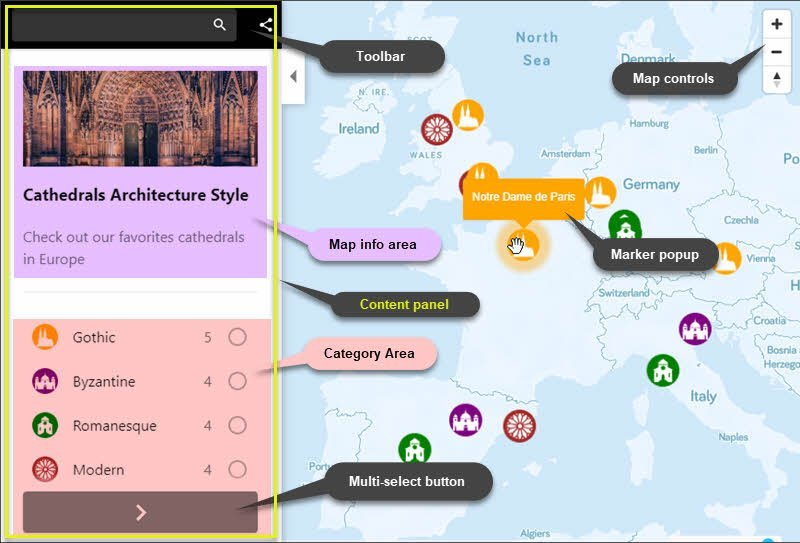
\includegraphics[width=\textwidth]{slike/map_example.png} %veličina u odnosu na širinu linije
			\caption{Primjer karte s tražilicom i prostorom za filtriranje.}
			\label{fig:primjerMape} %label mora biti drugaciji za svaku sliku
		\end{figure}
		
		Nakon što se prijavi, klijent može podijeliti svoje mišljenje o povoljnosti lokacije za pse. Pronalaskom željene lokacije (upis adrese ili imena u tražilicu) potvrđuje ili negira njezinu trenutnu oznaku, što ulazi u konačnu ocjenu te lokacije. Uz to, korisnik može stvoriti novu lokaciju koju će ocijeniti.\newline
		\underbar{Vlasnik obrta} ima mogućnosti korisnika vezane za pregled karte, traženje lokacija i filtriranje, ali nema mogućnost ocjenjivanja postojećih ili stvaranja novih lokacija za ocjenjivanje. Nadalje, plaćanjem pretplate pri registraciji on objavljuje vlastiti obrt na karti kako bi postao vidljiv svim korisnicima aplikacije. Iz tog razloga nužno unosi sve podatke koje korisnici vide:
		\begin{packed_item}
			\item {naziv}
			\item {adresa}
            \item {grad}
			\item {kontakt broj}
			\item {kratki opis obrta}
			\item {vrsta obrta (veterinarska ordinacija, salon za pse, dućan za pse, itd.)}
		\end{packed_item}
  
		Kao povlasticu, vlasnik svoj obrt može dodatno promovirati plaćanjem naknade uz već postojeću pretplatu. Isticanje se prezentira pojačavanjem markera na karti, ali i postavljanjem obrta u "Preporučeni obrti" prostoru gdje se u web aplikaciji preporučuju obrti vlasnika koji su dodatno uložili u isticanje. U slučaju da nema dodatno promoviranih obrta onda se u prostor "Preporučeni obrti" postavljaju najstariji obrti. U slučaju da obrti uopće ne postoje ispisuje se poruka "Trenutno nemamo preporučenih obrta.". \newline
  
		Sustav podržava rad više korisnika (registriran, neregistrirani) u stvarnom vremenu.
		
		
		
		
		\eject
		
	